\documentclass[14pt,titlepage]{extarticle}
\usepackage{ucs}
\usepackage[utf8x]{inputenc}
\usepackage[english,russian]{babel}
\usepackage{indentfirst}
\usepackage[usenames,dvipsnames]{color}
\usepackage{algorithm}
\usepackage{algorithmic}
\usepackage[pdftex]{graphicx}


\title{
  Анализ указателей и синонимов для многопоточных программ
}
\author{
  Владимир Парфиненко
}

% поля и размер текста
\textwidth=17cm
\oddsidemargin=-8pt
\topmargin=0pt
\headheight=0pt
\headsep=0pt
\textheight=23cm
\linespread{1.3}

\bibliographystyle{gost780u}

\graphicspath{{../images/}}

\floatname{algorithm}{Пример}
\renewcommand{\algorithmicrequire}{\textbf{Дано:}}

%\newcommand{\remark}[1]{}
\newcommand{\remark}[1]{\textcolor{green}{#1}}
\newcommand{\todo}[1]{\textcolor{red}{TODO: #1}}

\newenvironment{fresh}{\color{Blue}}{\color{black}}

\newcommand{\eng}[1]{{\English#1}}

\newcommand{\underscore}[1]{\hbox to#1{\hrulefill}}

\begin{document}

  %%%%%%%%%%%%%%%%%%%%%%%%%%%%%%%%%%%%%%%%%%%%%%%%
  %           Титульная страница
  %%%%%%%%%%%%%%%%%%%%%%%%%%%%%%%%%%%%%%%%%%%%%%%%
  \thispagestyle{empty}
  \begin {center}
    Министерство образования и науки

    Российской Федерации

    Федеральное агентство по образованию

    \vspace{0.3cm}

    Новосибирский государственный университет

    \vspace{0.3cm}

    Физический факультет

    Кафедра Автоматизации Физико-Технических Исследований

    \vspace {40mm}

    %Выпускная квалификационная работа бакалавра
    Февральский отчет

    \vspace {10mm}

    Парфиненко Владимир Владимирович

    \vspace {5mm}

    \textbf{АНАЛИЗ УКАЗАТЕЛЕЙ И СИНОНИМОВ\\ ДЛЯ МНОГОПОТОЧНЫХ ПРОГРАММ}

    \vspace {20mm}

    {\raggedleft

    Научный руководитель

    м.\,н.\,с.~ИСИ~СО~РАН, Павлов\,П.\,Е.

    \vspace {50mm}

    Новосибирск 2010}
  \end {center}


  \tableofcontents

  %%%%%%%%%%%%%%%%%%%%%%%%%%%%%%%%%%%%%%%%%%%%%%%%
  %                  Введение
  %%%%%%%%%%%%%%%%%%%%%%%%%%%%%%%%%%%%%%%%%%%%%%%%
  \newpage
  \section{Введение}

    Средства оптимизации программ нужны для получения высокой
    скорости исполнения программ или улучшения других характеристик программы.

    Под оптимизацией программ понимается преобразование программы в
    семантически эквивалентную, но более эффективную относительно некоторого
    заданного критерия.
    Преобразование программы $A$ в программу $B$ эквивалентно (или корректно),
    если из того, что программа $A$ выполнима на некотором наборе данных,
    следует, что и $B$ также выполнима на этом наборе и дает тот же результат,
    что и $A$.
    В общем случае задача проверки эквивалентности двух программ неразрешима,
    и не существует алгоритма, который по данной программе находил бы
    эквивалентную ей и оптимальную относительно заданного критерия
    \cite{kasjanov_translators}.

    Тем не менее существует набор известных оптимизирующих преобразований,
    таких, что корректность каждого из них гарантирует корректность их
    последовательного применения.
    И чтобы конкретное преобразование данной программы было корректным,
    необходимо выполнение некоторых условий. Например, чтобы иметь
    возможность убрать генерацию некоторой части программы, нужно быть
    увереным, что управление никогда не попадет в эту часть программы.
    Для получения подобной информации используют результаты статического
    анализа. Анализируя код программы, деляются выводы о тех или иных свойствах
    программы, необходимых для проведения преобразования.

    Статический анализ применяется не только для проверки
    корректности преобразований, но и в инструментах статического анализа
    кода программ, которые могут находить потенциальные ошибки и определять
    другие свойства программы без ее непосредственного исполнения.

    Существует множество видов статического анализа, и одним из них
    является анализ указателей и синонимов.

  %%%%%%%%%%%%%%%%%%%%%%%%%%%%%%%%%%%%%%%%%%%%%%%%%
  %%        Описание предметной области
  %%%%%%%%%%%%%%%%%%%%%%%%%%%%%%%%%%%%%%%%%%%%%%%%%
  \newpage
  \section{Описание предметной области}\label{section:overview}

    Анализ указателей~--- это один из видов статического анализа, который
    позволяет определить на какие объекты в памяти могут указывать выражения
    ссылочного типа в программе. Анализ синонимов похож на анализ указателей,
    его целью является определение, могут ли два разных выражения ссылаться
    на одно и то же место в памяти (такие выражения называют синонимами).

    Существует множество алгоритмов анализа указателей и синонимов,
    одним из них является алгоритм анализа, основанный на типах
    (\eng{Type-Based Alias Analysis}) \cite{diwan_tbaa},
    применимый для языков со строгой типизацией.
    В языках со строгой типизацией допускается присваивание переменной только
    значения, имеющего такой тип данных, что существует расширяющее
    преобразование к типу этой переменной.
    Например для языка Java, преобразование типа byte к типу int,
    преобразование ссылочного типа к его предку являются расширяющими
    преобразованиями, они безопасны и не требуют дополнительных действий
    на этапе исполнения.
    А преобразование типа double к типу float, преобразование типа
    Object к другому ссылочному типу являются сужающими, могут приводить к
    потере данных и требуют проверок на этапе исполнения.

    Простейшая реализация алгоритма основанного на типах полагается на то, что
    любая ссылочная переменная формального типа $T$ может указывать на любые
    объекты типа $T$ или его наследников. Такой алгоритм работает быстро,
    но обладает сравнительно низкой точностью.

    Для сравнения точности алгоритмов анализа указателей нам необходимо ввести
    некую меру точности. В качестве простой меры точности алгоритма можно
    использовать усредненное количество синонимов для переменных ссылочного
    типа, появляющихся в программе \cite{hind_pointer_analysis_not_solved_yet}.
    Понятно, что для «идеального» алгоритма анализа это число будет
    минимальным, а для самого консервативного алгоритма максимальным.

    Более точные алгоритмы анализа учитывают не только типы переменных,
    но и потоки данных в программе. Например, если существует только
    одно присваивание переменной нового объекта типа $T$, выделенного в куче,
    то можно гарантировать, что эта переменная может указывать только
    на этот объект.
    С присваиванием значения одной переменной другой переменной ситуация
    сложнее.
    \begin{algorithm}
      \caption{Сравнение \eng{subset-based} и \eng{equality-based} алгоритмов}
      \label{code:data_flow}
      \begin{algorithmic}[1]
        \STATE $b$ = new T()
        \STATE $c$ = new T()
        \STATE $a$ = $b$
        \STATE $a$ = $c$
      \end{algorithmic}
    \end{algorithm}
    Рассмотрим пример \ref{code:data_flow}.
    Для удобства, цели указателя, то есть множество объектов, на которые может
    указывать указатель $p$ (или переменная ссылочного типа), обозначим как
    $Pts(p)$ (англ. \eng{Points-to set}).
    Учитывая строки 1 и 2, для переменных $b$ и $c$ мы можем точно определить
    множество объектов, на которые они указывают,
    \[Pts(b) = \{O_1\}, Pts(c) = \{O_2\},\] где $O_1$ и $O_2$ уникальные
    объекты в куче. То есть мы учли поток данных от оператора new,
    вернувшего новый объект, в переменную.

    Интерпретировать присваивание $a = b$ можно двумя способами,
    и алгоритмы анализа разбиваются на два типа по этому признаку:
    \begin{itemize}
      \item алгоритмы первого типа накладывают ограничение
            $Pts(a) \supset Pts(b)$ (\eng{subset-based} алгоритмы),
      \item алгоритмы второго типа накладывают ограничение
            $Pts(a) = Pts(b)$ (\eng{equality-based} алгоритмы).
    \end{itemize}
    Первый тип алгоритмов более точен, в то время как второй быстрее
    \cite{steensgaard}. Возвращаясь к нашему примеры, \eng{subset-based}
    алгоритм получит, что
    \[Pts(a) = \{O_1, O_2\}, Pts(b) = \{O_1\}, Pts(c) = \{O_2\},\]
    а \eng{equality-based}
    \[Pts(a) = Pts(b) = Pts(c) = \{O_1, O_2\}.\]

    \begin{fresh}

    Также алгоритм может учитывать поток управления в программе. Рассмотрим
    пример \ref{code:control_flow}.
    \begin{algorithm}
      \caption{Сравнение чувствительного и нечувствительного к потоку
               управления алгоритма}
      \label{code:control_flow}
      \begin{algorithmic}[1]
        \STATE $a$ = new T()
        \STATE $b$ = new T()
        \STATE $c$ = new T()
        \STATE $a$ = $b$
        \STATE $b$ = $c$
        \STATE $c$ = $a$
      \end{algorithmic}
    \end{algorithm}
    Чувствительный к потоку управления анализ получит следующие данные после
    3-ей строки
    \[\textrm{строка 3}:
        Pts(a) = \{O_a\}, Pts(b) = \{O_b\}, Pts(c) = \{O_c\}.\]
    Далее, при анализе 4-ой строки, алгоритм поймет что $Pts(a) = \{O_b\}$,
    фактически, не только сгенерировав информацию о том, что $a$ может
    указывать на $O_b$, но и уничтожив информацию о том, что $a$ может
    указывать на $O_a$.
    Проведя аналогичные рассуждения к концу программы получатся следующие
    результаты:
    \[\textrm{строка 6}:
        Pts(a) = \{O_b\}, Pts(b) = \{O_c\}, Pts(c) = \{O_b\}.\]
    Получается, что такой алгоритм должен хранить информацию о состоянии целей
    указателей для каждой инструкции отдельно.

    Нечувствительный к потоку управления анализ воспринимает программу не как
    последовательность инструкций, а как их неупорядоченный набор.
    Для указанного примера такой анализ получит следующее
    \[Pts(a) = Pts(b) = Pts(c) = \{O_a, O_b, O_c\}.\]
    Этот результат не является точным, но зато полученная информация верна для
    любой точки программы и может хранится в единственном экземпляре.

    \end{fresh}

    Рассмотрим, как алгоритм анализа может обрабатывать вызовы
    функций и процедур на примере \ref{code:interprocedural}.
    \begin{algorithm}
      \caption{Демонстрация работы межпроцедурного алгоритма}
      \label{code:interprocedural}
      \begin{algorithmic}[1]
        \STATE function foo($x$, $y$) \{ return $x$ \}
        \STATE $b$ = new T()
        \STATE $c$ = new T()
        \STATE $a$ = foo($b$, $c$)
      \end{algorithmic}
    \end{algorithm}
    Наша задача понять, чему равно $Pts(a)$.
    Алгоритмы анализа можно разделить на две категории, в зависимости от того,
    как они обрабатывают вызовы функций:
    \begin{itemize}
      \item межпроцедурные алгоритмы анализа могут сначал проанализировать
            тело вызываемой функции, и затем учесть результат при обработке
            вызова,
      \item внутрипроцедурные алгоритмы рассматривают вызов функции в наиболее
            консервативном предположении: может быть возвращен либо один из
            параметров, либо любой глобальный объект, либо новый объект.
    \end{itemize}
    Понятно, что первый тип алгоритмов дает более точные результаты,
    а второй потребляет меньше памяти и работает быстрее
    \cite[с.~117]{andersen}.
    В нашем примере межпроцедурный алгоритм анализа, проанализировав функцию
    foo, запоминает, что для нее выполнено следующее условие на возвращаемое
    значение
    \[Pts(retval) = Pts(x),\]
    и тогда может сделать вывод, что \[Pts(a) = Pts(b) = \{O_1\}.\]
    В такой же ситуации внутрипроцедурный алгоритм анализа обязан сделать
    консервативное предположение
    \[Pts(a) = Pts(b) \cup Pts(c) = \{O_1, O_2\}.\]

  %%%%%%%%%%%%%%%%%%%%%%%%%%%%%%%%%%%%%%%%%%%%%%%%
  %             Постановка задачи
  %%%%%%%%%%%%%%%%%%%%%%%%%%%%%%%%%%%%%%%%%%%%%%%%
  \newpage
  \section{Постановка задачи}

    Целью данной работы является изучение существующих алгоритмов анализа
    указателей, последующая разработка внутрипроцедурного алгоритма и
    внутренного представления для использования в оптимизирующем
    статическом компиляторе Java программ
    \eng{Excelsior Research Virtual Machine (Excelsior~RVM)}
    с учетом приведенных ниже требований.

    Алгоритм анализа должен учитывать следующие особенности языка Java:
    \begin{itemize}
      \item наличие строгой типизации,
      \item отсутствие адресной арифметики,
      \item отсутствие указателей на указатели.
    \end{itemize}
    Именно эти особенности отличают язык Java от языка C при рассмотрении
    анализа указателей, для которого были
    спроектированны классические алгоритмы анализа указателей
    Стинсгарда \cite{steensgaard} и Андерсена \cite{andersen}.

    В свзяи с широким распространением многопоточных программ,
    алгоритм анализа необходимо адаптировать для применения к
    многопоточным программам согласно спецификации JVM, которая имеет
    строгое и подробное описание модели памяти (Java Memory Model)
    \cite{manson_jmm}.

    Кроме того внутреннее представление программы должно быть адаптировано,
    для хранения результатов анализа указателей, и предоставлять удобный
    интерфейс для получения этих результатов другими алгоритмами статического
    анализа.

    Для достижения поставленной цели необходимо:
    \begin{itemize}
      \item изучив существующие алгоритмы анализа указателей, выбрать
            подходящий внутрипроцедурный алгоритм и адаптировать его
            для анализа многопоточных программ на языке Java,
      \item адаптировать существующее внутреннее представление программы для
            хранения результатов анализа указателей,
      \item реализовать алгоритм и внутреннее представление для оптимизирующего
            статического компилятора Java программ \eng{Excelsior RVM}.
    \end{itemize}

  %%%%%%%%%%%%%%%%%%%%%%%%%%%%%%%%%%%%%%%%%%%%%%%%
  %
  %%%%%%%%%%%%%%%%%%%%%%%%%%%%%%%%%%%%%%%%%%%%%%%%
  \begin{fresh}
  \newpage
  \section{Описание алгоритма анализа}

    \subsection{Система типов языка Java}

    \subsection{Внутреннее представление и SSA-форма}

      В процессе компиляции программа на исходном языке программирования
      переводится в, так называемое, внутреннее представление программы
      (англ. \eng{internal representation, IR}), на котором работают
      алгоритмы анализа и на котором проводятся все оптимизации. Будем
      рассматривать внутреннее представление тела функции, заданное в виде
      графа управления (англ. \eng{control flow graph, CFG}). CFG~--- это
      ориентированный граф, в котором вершинам соответствуют последовательности
      операторов программы, а дугам~--- переходы из конца одной
      последовательности операторов в начало другой. Такие последовательности
      операторов, являющиеся вершинами, назовем линейными участками. В конце
      каждого линейного участка присутствует оператор перехода, который
      передает управление по одной из дуг, выходящих из данной вершины CFG.

      Будем говорить, что программа находится в SSA-форме (\eng{Static Single
      Assignment}), если существует не более одного присваивания каждой
      переменной. В SSA-форме вводится дополнительная операция слияния значений
      переменных, так называемая $\phi$-функция. Пусть в CFG существует вершина
      $N$, такая что в нее входит больше одной дуги из вершин
      $N_1$, ..., $N_K$, назовем такую вершину точкой слияния. Тогда в $N$
      будут располагаться следующие вызовы $\phi$-функций
      \[ v = \phi(v_1, ..., v_K), \]
      для всех переменных $v$ требующих слияния.
      Семантика данной операции заключается в присваивании переменной $v$
      значения переменной $v_i$, соответствующего вершине $N_i$, из которой
      управление пришло в $N$. В случае CFG, приведенного на рисунке
      \ref{fig:cfg_with_phi}, переменной $a_3$ будет присвоено значение 5 или
      7, если управление придет в нижнюю вершину через левую или правую
      вершину, соответственно.

      \begin{figure}[!htb]
        \center{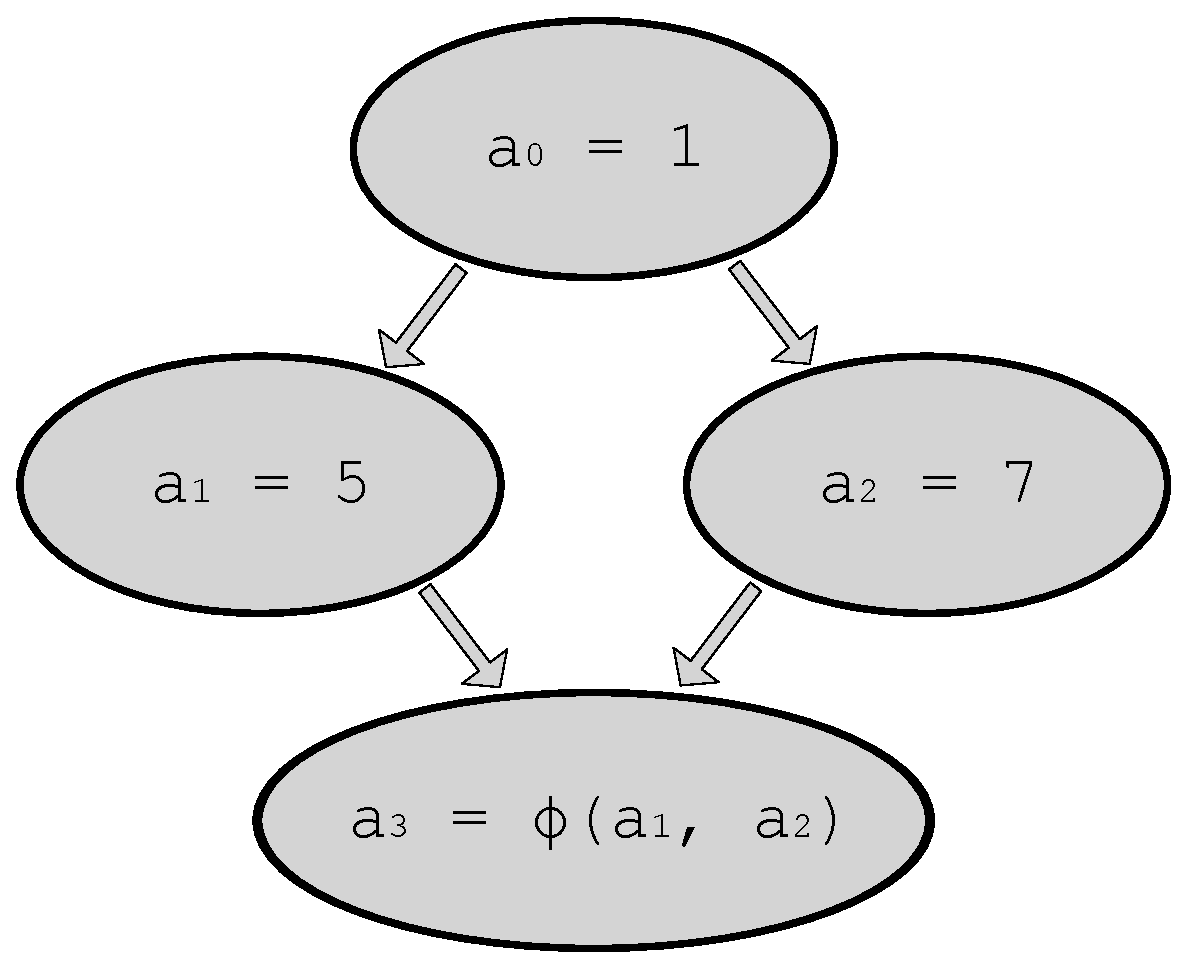
\includegraphics[width=80mm]{phi_func}}
        \caption{Пример CFG с $\phi$-функцией}
        \label{fig:cfg_with_phi}
      \end{figure}

      Для преобразования внутреннего представления программы в SSA-форму и
      обратно существуют эффективные алгоритмы \cite{ssa}. В то же время
      многие виды анализа и многие оптимизации проще и эффективнее проводить
      именно на внутреннем представлении в SSA-форме, поэтому его и будем
      использовать для проведения анализа указателей.

    \subsection{Операции и их семантика}

      Сначала определим точно, что может быть указателем в языке Java и
      подобных ему. В C-подобных языках допустимы переменные, поля объектов,
      элементы масивов, указывающие на:
      \begin{itemize}
        \item объекты в куче,
        \item объекты на стеке,
        \item другие переменные,
        \item функции.
      \end{itemize}
      В Java-подобных языках ситуациях существенно отличается, так как целью
      указателя может быть только объект, находящийся в куче. Так же
      отсутствует адресная арифметика, за счет чего ссылка на объект не может
      появиться неявно.

      Для проведения анализа указателей необходимо учитывать не все операции
      допустимые в языке, а лишь те, которые могут изменять цели указателей.
      Необходимо рассматривать лишь следующие инструкции ($a$, $b$, $c$~---
      переменные или формальные параметры ссылочного типа):
      \begin{center}
        \begin{tabular}{|l|p{120mm}|}\hline
          \textbf{Инструкция} & \textbf{Описание}\\ \hline

          $a$ = $b$
          & присваивание значения $b$ переменной $a$ \\ \hline

          $a$ = null
          & указание, что $a$ не указывает ни на один объект \\ \hline

          $a$ = new $T$
          & создание нового объекта типа $T$ в куче \\ \hline

          $a$ = $b$.$f$
          & чтение поля объекта, на который ссылается $b$ \\ \hline

          $b$.$f$ = $a$
          & запись в поле объекта, на который ссылается $b$ \\ \hline

          $a$ = $T$.$f$
          & чтение статического поля класса $T$ \\ \hline

          $T$.$f$ = $a$
          & запись в статическое поле класса $T$ \\ \hline

          $a$ = $b$[\ldots]
          & чтение элемента массива $b$ \\ \hline

          $b$[\ldots] = $a$
          & запись в элемент массива $b$ \\ \hline

          $a$ = ($T$)$b$
          & преобразования значения переменной $b$ к типу $T$ \\ \hline

          $a$ = foo($b$, \ldots)
          & вызов функции foo, возращающей значение ссылочного типа \\ \hline

          foo($b$, \ldots)
          & вызов функции foo, либо не возращающей значение, либо возвращающей значение примитивного типа \\ \hline
        \end{tabular}
      \end{center}

      Так как для алгоритма анализа сложно определить индекс элемента при
      чтении и записи в массив, удобно рассматривать массив как объект с
      единственным полем $elements$, из которого читаются и в которое
      записываются все значения при обращении к элементам массива.

      При преобразовании $a$ = ($T$)$b$ в случае неудачного преобразования
      значения переменной $b$ к типу $T$ будет выброшено исключение во время
      исполнения, поэтому в рамках анализа, можно считать что переменная $a$
      может указывать только на объекты, совместимые по присваиванию с типом
      $T$.

      При вызове другой функции нужно понимать, что вызванная функция может
      изменять цели полей переданных параметров и полей статических переменных.


    \subsection{Тип алгоритма}

      Необходимо определиться с характеристиками алгоритма анализа
      подходящего для нашей задачи. Описание основных характеристик уже было
      приведено в разделе~\ref{section:overview}.

    \subsubsection{\eng{Subset-based} алгоритм анализа}

      При выборе между \eng{subset-based} и \eng{equality-based} алгоритмом
      анализа, необходимо выбрать, что важнее для конечного алгоритма:
      точность или скорость работы, соответственно. Проведенные эксперименты
      показывают \cite{shapiro_fast_and_accurate}, что на небольших программах
      (до 3000 строк), время работы обоих алгоритмов анализа примерно
      одинаково, но точность у \eng{subset-based} алгоритма значительно выше.
      Забегая вперед, отмечу, что алгоритм будет применятся для
      внутрепроцедурного анализа, и поэтому, выбирая \eng{subset-based}
      алгоритм, выигрыш в точности анализа будет весомым, а потери во времени
      работы алгоритма незначительны, так как отдельный метод программы
      разумно отнести к «небольшим программам».

    \subsubsection{Нечувствительный к потоку алгоритм анализ}

      Рассмотрим чувствительность алгоритма анализа указателей к потоку
      управления.  Если алгоритм анализа чувствителен к потоку управления, он
      может давать более точные результаты, набор целей указателей для
      конкретной точки в программе
      \cite[с.~57]{hind_pointer_analysis_not_solved_yet}, но и этих наборов
      получается, при простейшем подходе, по одному на каждую инструкцию
      программы, что приводит к дополнительному потреблению памяти алгоритмом
      анализа. Рассмотрим подробнее, за счет чего у такого алгоритма получается
      более точный результат. При присваивании $a = b$ не только генерируется
      информация об указании переменной $a$ на все объекты, на которые может
      указывать переменная $b$, но и уничтожается предыдущая информация о целях
      переменной $a$, за счет этого множество целей переменной $a$ содержит
      меньше неактуальной для этой точки программы информации. Но похожего
      результата можно достичь и другим путем, используя SSA-форму для
      внутреннего представления.

      Рассмотрим работу алгоритма нечувствительного к потоку на
      примере \ref{code:ssa_precision}
      (это пример \ref{code:control_flow} переведенный в SSA-форму).
      \begin{algorithm}
        \caption{Повышение точности за счет использования SSA-формы}
        \label{code:ssa_precision}
        \begin{algorithmic}[1]
          \REQUIRE $x_0$, $x_1$, ..., $x_i$~--- версии одной переменной $x$
          \STATE $a_0$ = new T()
          \STATE $b_0$ = new T()
          \STATE $c_0$ = new T()
          \STATE $a_1$ = $b_0$
          \STATE $b_1$ = $c_0$
          \STATE $c_1$ = $a_1$
        \end{algorithmic}
      \end{algorithm}
      Так как присутствует только одно присваивание каждой переменной, легко
      получается следующий результат:
      \[Pts(a_0) = \{O_a\}, Pts(b_0) = \{O_b\}, Pts(c_0) = \{O_c\},\]
      \[Pts(a_1) = \{O_b\}, Pts(b_1) = \{O_c\}, Pts(c_1) = \{O_b\}.\]
      Как было показано в разделе \ref{section:overview} чувствительный к
      потоку алгоритм анализа дает идентичный результат для конечной точки
      примера \ref{code:control_flow} (учитывая, что для конечной точки
      программы $a = a_1$, $b = b_1$, $c = c_1$):
      \[Pts(a) = \{O_b\}, Pts(b) = \{O_c\}, Pts(c) = \{O_b\}.\]
      Получается, что чувствительный к потоку анализ не дает выигрыша в
      точности при использования SSA-формы, это связано с тем, что не
      происходит того «уничтожения предыдущей информации о целях переменной»,
      так как неактуальная информация о целях предыдущих версий переменной не
      переходит в последующие версии.

      В итоге получается, что чувствительный к потоку алгоритм и алгоритм
      анализа, работающий на SSA-форме внутреннего представления, дают
      одинаково точные результаты и каждый требует дополнительной памяти, либо
      на хранение набора целей указателей для точек программы, либо на хранение
      целей указателей для всех версий переменной. Но необходимо заметить, что
      большинство современных компиляторов уже используют SSA-форму для
      внутреннего представления программы, и следовательно, при прочих равных
      нет смысла использовать чувствительный к потоку алгоритм анализа.

    \subsubsection{Внутрипроцедурный алгоритм анализа}

      Межпроцедурные алгоритмы анализа указателей сравнительно сложны для
      реализации, хотя и дают более точные результаты. Тем более реализация
      подобного алгоритма для таких языков как Java, где каждый нестатический
      метод является виртуальным, выходит за рамки моей квалификационной
      работы. Но стоит понимать, что до вызова алгоритма анализа уже может быть
      проведена оптимизация открытой подстановки методов, что позволит смягчить
      последствия от отсутствия межпроцедурного анализа.

    \subsection{Описание алгоритма анализа для однопоточных программ}

    \subsection{Модель памяти языка Java}

    \subsection{Описание алгоритма анализа для многопоточных программ}

  \end{fresh}

  %%%%%%%%%%%%%%%%%%%%%%%%%%%%%%%%%%%%%%%%%%%%%%%%
  %             Список литературы
  %%%%%%%%%%%%%%%%%%%%%%%%%%%%%%%%%%%%%%%%%%%%%%%%
  \newpage
  \addcontentsline{toc}{section}{Список литературы}
  %\begin{flushleft}
    \bibliography{../../biblio}
  %\end{flushleft}

  %%%%%%%%%%%%%%%%%%%%%%%%%%%%%%%%%%%%%%%%%%%%%%%%
  %               План график
  %%%%%%%%%%%%%%%%%%%%%%%%%%%%%%%%%%%%%%%%%%%%%%%%
  \newpage
  \thispagestyle{empty}
  \pagestyle{empty}
  \section*{План-график}

    \todo{обновить}
    \begin{center}
      \begin{tabular}{|p{10.5cm}|c|c|}\hline
        \textbf{Задача}                       &\textbf{Время} & \textbf{Срок}\\
        \hline
        Изучение существующих алгоритмов анализа указателей
                                              & 2 месяца    & 31 ноября \\
        \hline
        Реализация прототипа алгоритма анализа для однопоточных программ
                                              & 1,5 месяца  & 15 января \\
        \hline
        Реализация прототипа алгоритма анализа для многопоточных программ
                                              & 1 месяц     & 15 февраля \\
        \hline
        Реализация алгоритма анализа и преобразование внутреннего представления
        в оптимизирующем Java компиляторе Excelsior RVM
                                              & 1,5 месяца  & 31 марта \\
        \hline
      \end{tabular}
    \end{center}



  %%%%%%%%%%%%%%%%%%%%%%%%%%%%%%%%%%%%%%%%%%%%%%%%
  %                  Оценки
  %%%%%%%%%%%%%%%%%%%%%%%%%%%%%%%%%%%%%%%%%%%%%%%%
  \newpage
  \thispagestyle{empty}
  \pagestyle{empty}
  \section*{Оценка за февральский отчёт}

    Руководитель: \underscore{1cm} (из 10 баллов).
    Подпись: \underscore{3cm} (Павлов\,П.\,Е.)

    \vspace{0.5cm}
    Преподаватель: \underscore{1cm}
\end{document}

